\documentclass[journal,12pt,twocolumn]{IEEEtran}
%
\usepackage{setspace}
\usepackage{gensymb}
\usepackage{xcolor}
\usepackage{caption}
\usepackage{circuitikz}
%\usepackage{subcaption}
%\doublespacing
\singlespacing
\usepackage{float}
%\usepackage{graphicx}
%\usepackage{amssymb}
%\usepackage{relsize}
\usepackage[cmex10]{amsmath}
\usepackage{mathtools}
%\usepackage{amsthm}
%\interdisplaylinepenalty=2500
%\savesymbol{iint}
%\usepackage{txfonts}
%\restoresymbol{TXF}{iint}
%\usepackage{wasysym}
\usepackage{hyperref}
\usepackage{amsthm}
\usepackage{mathrsfs}
\usepackage{txfonts}
\usepackage{stfloats}
\usepackage{cite}
\usepackage{cases}
\usepackage{subfig}
%\usepackage{xtab}
\usepackage{longtable}
\usepackage{multirow}
%\usepackage{algorithm}
%\usepackage{algpseudocode}
%\usepackage{enumerate}
\usepackage{enumitem}
\usepackage{mathtools}
%\usepackage{iithtlc}
%\usepackage[framemethod=tikz]{mdframed}
\usepackage{listings}
\let\vec\mathbf


%\usepackage{stmaryrd}


%\usepackage{wasysym}
%\newcounter{MYtempeqncnt}
\DeclareMathOperator*{\Res}{Res}
%\renewcommand{\baselinestretch}{2}
\renewcommand\thesection{\arabic{section}}
\renewcommand\thesubsection{\thesection.\arabic{subsection}}
\renewcommand\thesubsubsection{\thesubsection.\arabic{subsubsection}}

\renewcommand\thesectiondis{\arabic{section}}
\renewcommand\thesubsectiondis{\thesectiondis.\arabic{subsection}}
\renewcommand\thesubsubsectiondis{\thesubsectiondis.\arabic{subsubsection}}

%\renewcommand{\labelenumi}{\textbf{\theenumi}}
%\renewcommand{\theenumi}{P.\arabic{enumi}}

% correct bad hyphenation here
\hyphenation{op-tical net-works semi-conduc-tor}

\lstset{
language=Python,
frame=single, 
breaklines=true,
columns=fullflexible
}



\begin{document}
%

\theoremstyle{definition}
\newtheorem{theorem}{Theorem}[section]
\newtheorem{problem}{Problem}
\newtheorem{proposition}{Proposition}[section]
\newtheorem{lemma}{Lemma}[section]
\newtheorem{corollary}[theorem]{Corollary}
\newtheorem{example}{Example}[section]
\newtheorem{definition}{Definition}[section]
%\newtheorem{algorithm}{Algorithm}[section]
%\newtheorem{cor}{Corollary}
\newcommand{\BEQA}{\begin{eqnarray}}
\newcommand{\EEQA}{\end{eqnarray}}
\newcommand{\define}{\stackrel{\triangle}{=}}
\newcommand{\myvec}[1]{\ensuremath{\begin{pmatrix}#1\end{pmatrix}}}
\newcommand{\mydet}[1]{\ensuremath{\begin{vmatrix}#1\end{vmatrix}}}

\bibliographystyle{IEEEtran}
%\bibliographystyle{ieeetr}

\providecommand{\nCr}[2]{\,^{#1}C_{#2}} % nCr
\providecommand{\nPr}[2]{\,^{#1}P_{#2}} % nPr
\providecommand{\mbf}{\mathbf}
\providecommand{\pr}[1]{\ensuremath{\Pr\left(#1\right)}}
\providecommand{\qfunc}[1]{\ensuremath{Q\left(#1\right)}}
\providecommand{\sbrak}[1]{\ensuremath{{}\left[#1\right]}}
\providecommand{\lsbrak}[1]{\ensuremath{{}\left[#1\right.}}
\providecommand{\rsbrak}[1]{\ensuremath{{}\left.#1\right]}}
\providecommand{\brak}[1]{\ensuremath{\left(#1\right)}}
\providecommand{\lbrak}[1]{\ensuremath{\left(#1\right.}}
\providecommand{\rbrak}[1]{\ensuremath{\left.#1\right)}}
\providecommand{\cbrak}[1]{\ensuremath{\left\{#1\right\}}}
\providecommand{\lcbrak}[1]{\ensuremath{\left\{#1\right.}}
\providecommand{\rcbrak}[1]{\ensuremath{\left.#1\right\}}}
\theoremstyle{remark}
\newtheorem{rem}{Remark}
\newcommand{\sgn}{\mathop{\mathrm{sgn}}}
\providecommand{\abs}[1]{\left\vert#1\right\vert}
\providecommand{\res}[1]{\Res\displaylimits_{#1}} 
\providecommand{\norm}[1]{\lVert#1\rVert}
\providecommand{\mtx}[1]{\mathbf{#1}}
\providecommand{\mean}[1]{E\left[ #1 \right]}
\providecommand{\fourier}{\overset{\mathcal{F}}{ \rightleftharpoons}}
\providecommand{\ztrans}{\overset{\mathcal{Z}}{ \rightleftharpoons}}

%\providecommand{\hilbert}{\overset{\mathcal{H}}{ \rightleftharpoons}}
\providecommand{\system}{\overset{\mathcal{H}}{ \longleftrightarrow}}
	%\newcommand{\solution}[2]{\textbf{Solution:}{#1}}
\newcommand{\solution}{\noindent \textbf{Solution: }}
\providecommand{\dec}[2]{\ensuremath{\overset{#1}{\underset{#2}{\gtrless}}}}
\numberwithin{equation}{section}
%\numberwithin{equation}{subsection}
%\numberwithin{problem}{subsection}
%\numberwithin{definition}{subsection}
\makeatletter
\@addtoreset{figure}{problem}
\makeatother

\let\StandardTheFigure\thefigure
%\renewcommand{\thefigure}{\theproblem.\arabic{figure}}
\renewcommand{\thefigure}{\theproblem}


%\numberwithin{figure}{subsection}

\def\putbox#1#2#3{\makebox[0in][l]{\makebox[#1][l]{}\raisebox{\baselineskip}[0in][0in]{\raisebox{#2}[0in][0in]{#3}}}}
     \def\rightbox#1{\makebox[0in][r]{#1}}
     \def\centbox#1{\makebox[0in]{#1}}
     \def\topbox#1{\raisebox{-\baselineskip}[0in][0in]{#1}}
     \def\midbox#1{\raisebox{-0.5\baselineskip}[0in][0in]{#1}}

\vspace{3cm}

\title{ 
%\logo{
%}
Circuits and Transforms
%	\logo{Octave for Math Computing }
}
%\title{
%	\logo{Matrix Analysis through Octave}{\begin{center}\includegraphics[scale=.24]{tlc}\end{center}}{}{HAMDSP}
%}



\author{ Mannem Charan AI21BTECH11019 %<-this  stops a space
}
\maketitle


\tableofcontents


\renewcommand{\thefigure}{\theenumi}
\renewcommand{\thetable}{\theenumi}



\bigskip

\begin{abstract}
This manual provides a simple introduction to Transforms
\end{abstract}

 \section{Definitions}
\begin{enumerate}[label=\arabic*.,ref=\thesection.\theenumi]
\numberwithin{equation}{section}
\numberwithin{figure}{section}
\item The unit step function is 
\begin{align}
u(t) =
\begin{cases}
1 & t > 0
\\
	\frac{1}{2} & t = 0
\\
0 & t < 0
\end{cases}
\end{align}
\item The Laplace transform of $g(t)$ is defined as 
\begin{align}
	G(s) = \int_{-\infty}^{\infty} g(t) e^{-st}\, dt\label{eq:laplace}
\end{align}
 \end{enumerate}

 \section{Laplace Transform}
\begin{enumerate}[label=\arabic*.,ref=\thesection.\theenumi]
\numberwithin{equation}{section}
\item In the circuit, the switch S is connected to position P for a long time so that the charge on the capacitor
	becomes $q_1 \, \mu C$. Then S is switched to position Q.  After a long time, the charge on the capacitor is
		$q_2 \, \mu C$.
		\begin{figure}[!ht]
			\centering
			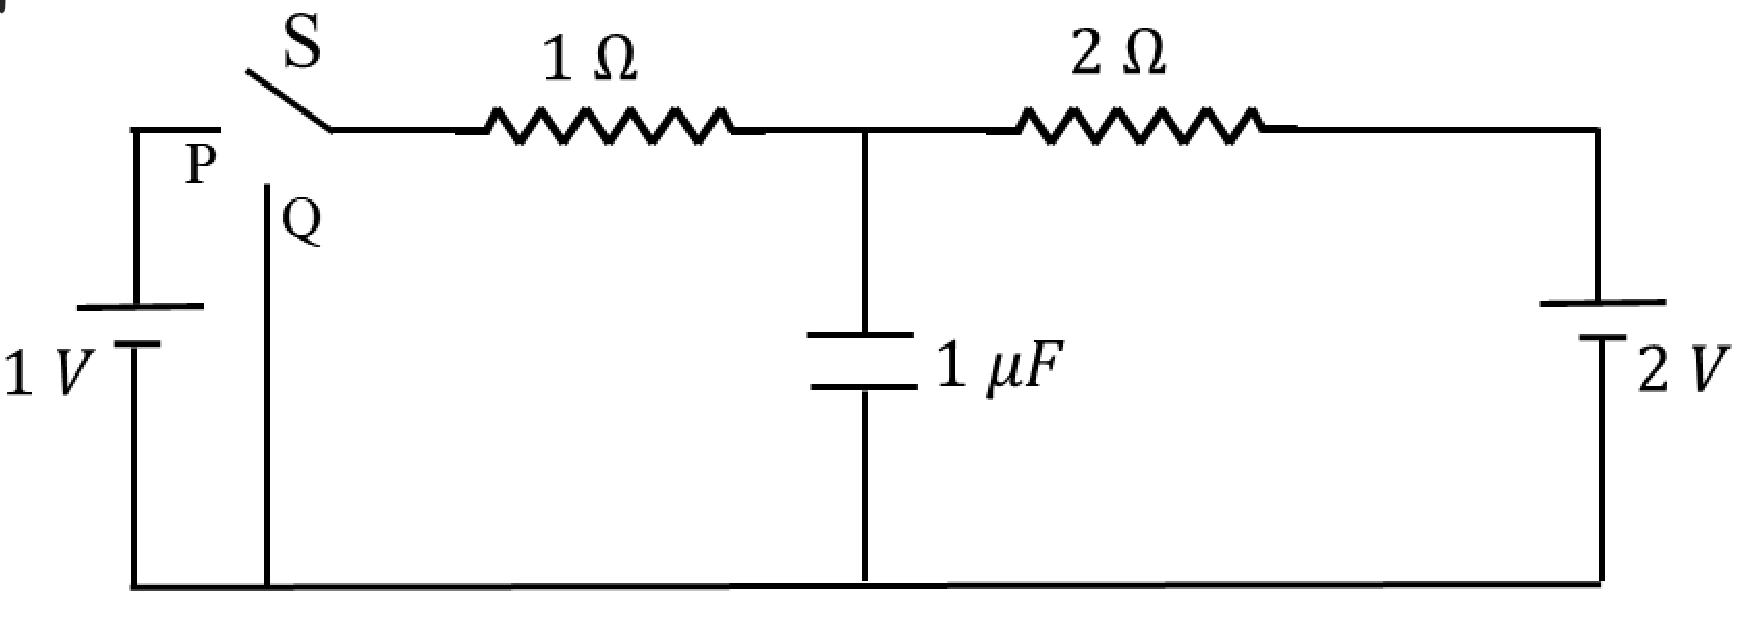
\includegraphics[width=\columnwidth]{Figs/ckt.jpg}
			\caption{}
			\label{fig:ckt}
\end{figure}
\item Draw the circuit using latex-tikz. \\
 \solution 
 \begin{figure}[!ht]
	  \begin{center}
	   \begin{circuitikz}
            \draw (0,0) 
             to [short] (8,0)
	     ;
	    \draw (8,3)
	     to [battery1,l_ = $2V$](8,0)
	     ;
	     \draw (0,3)
	     to [battery1,l_ = $1V$](0,0)
	     ;
	     \draw (8,3)
             to [R = $2\Omega$](4,3) 
	     to [R = $1\Omega$](1,3)
	     to [nos, l_ = S,mirror] (0,3) node[label = {left:P}]{}
	     ;
	     \draw (4,3)
	     to [C =  1 $\mu F$](4,0);
	     \draw (0.8,0)
	      to [short](0.8,2.7) node[label = {right:Q}]{}
	      
	      ;
	   \end{circuitikz}
   \end{center}
   \caption{Circuit diagram of the question}
   \label{circt-1}
\end{figure}
\item Find $q_1$.\\
 \solution Since the switch S is closed for a long time at P, the circuit at steady state looks like,
    \begin{figure}[!ht]
	 \begin{center}
	  \begin{circuitikz}
	  \draw (0,0) 
             to [short] (8,0)
	     ;
	    \draw (8,3)
	     to [battery1,i_ = $i$,l_ = $2V$](8,0)
	     ;
	     \draw (0,3)
	     to [battery1,l_ = $1V$](0,0)
	     ;
	     \draw (8,3)
             to [R = $2\Omega$](4,3) 
	     to [R = $1\Omega$](1,3)
	     to [short](0,3)
	     ;
	     \draw (4,3)
	     to [short,*-o](4,1.75)node[left]{$+$};
	     \draw (4,0)
	     to [short,*-o](4,1.25)node[left]{$-$};
	  \end{circuitikz}
	  \end{center}
     \end{figure}
	     Now if we apply KVL,
	 \begin{align}
		 2 - 2i-i -1 &=0 \\
	  \implies i &= \frac{1}{3}
	 \end{align}
	 The potential difference across capacitor is,
	  \begin{align}
		  V_{C} &= 2 - 2i \\
		        &= \frac{4}{3}
	  \end{align}
       Therefore the charge on capacitor will be,
        \begin{align}
	  q_{1} &= \frac{4}{3} \mu F
	 \end{align}
     \item Show that the Laplace transform of $u(t)$ is $\frac{1}{s}$ and find the ROC.\\
	     \solution From $\ref{eq:laplace}$ we can write laplace transform of unit step function $u(t)$ as,
	      \begin{align}
                 \mathcal{L}\cbrak{u(t)} &= \int_{-\infty}^{\infty}u(t)e^{-st}dt \\
					 &= \int_{0}^{\infty}e^-stdt \\
					 &=  \sbrak{\frac{e^{-st}}{-s}}_{0}^{\infty} 
	      \end{align}
	      For the laplace transform to exist,$Re\brak{s} >0$ using that
	       \begin{align}
		       \mathcal{L}\cbrak{u(t)} &= \frac{1}{s} \text{with ROC $Re\brak{s} >0$}
               \end{align}
	       The ROC plot looks like $\ref{Fig:ROC_1}$,
	 \begin{figure}[!ht]
	    \centering
	    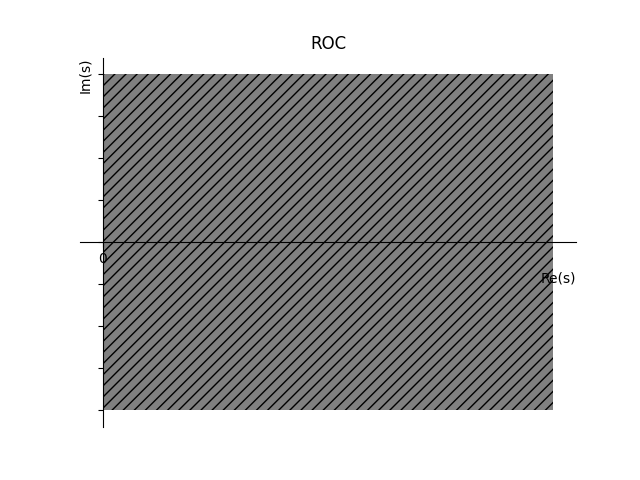
\includegraphics[width = \columnwidth]{Figs/2.4.png}
	    \caption {ROC of laplace transform of $u(t)$}
	    \label{Fig:ROC_1}
           \end{figure}
        \item Show that 
		\begin{align}
			e^{-at}u(t) \system{L} \frac{1}{s+a}, \quad a > 0
		\end{align}
		and find the ROC. \\
	 \solution The laplace transform will be,
	   \begin{align}
		   \mathcal{L}\cbrak{e^{-at}u(t)} &= \int_{-\infty}^{\infty}e^{-\brak{a+s}t}u(t)dt \\
						  &= \int_{0}^{\infty}e^{-\brak{a+s}t} dt \\
						  &= \sbrak{\frac{e^{-\brak{a+s}t}}{-\brak{a+s}}}_{0}^{\infty}
	   \end{align}
	   Now for the integral to exist,
	    \begin{align}
		    Re\brak{s+a} > 0 \\
		    Re\brak{s} > -a
	    \end{align}
	    So the ROC will be $Re\brak{s} > -a$ and with that ROC, 
	     \begin{align}
		     \mathcal{L}\cbrak{e^{-at}u(t)} &= \frac{1}{a+s}
	     \end{align}
	     And the ROC plot looks like $\ref{Fig:ROC_2}$,
	      \begin{figure}
	       \centering
	       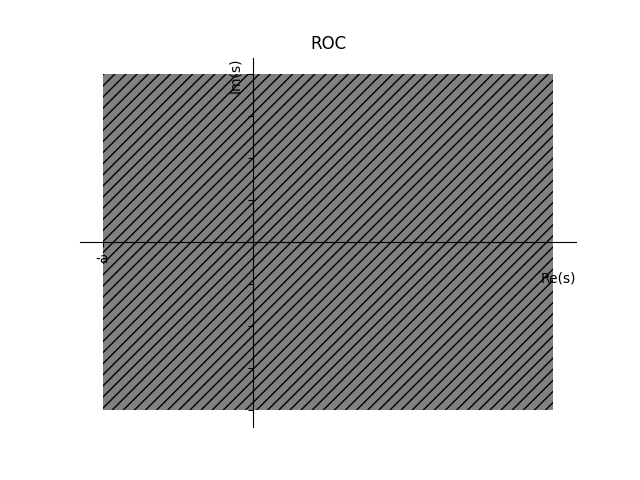
\includegraphics[width = \columnwidth]{Figs/2.5.png}
	       \caption{ROC of laplace transform of $e^{-at}u\brak{t}$}
	       \label{Fig:ROC_2}
	      \end{figure}
	\item Now consider the following resistive circuit transformed from 
			Fig. $\ref{fig:ckt}$
		\begin{figure}[!ht]
			\centering
			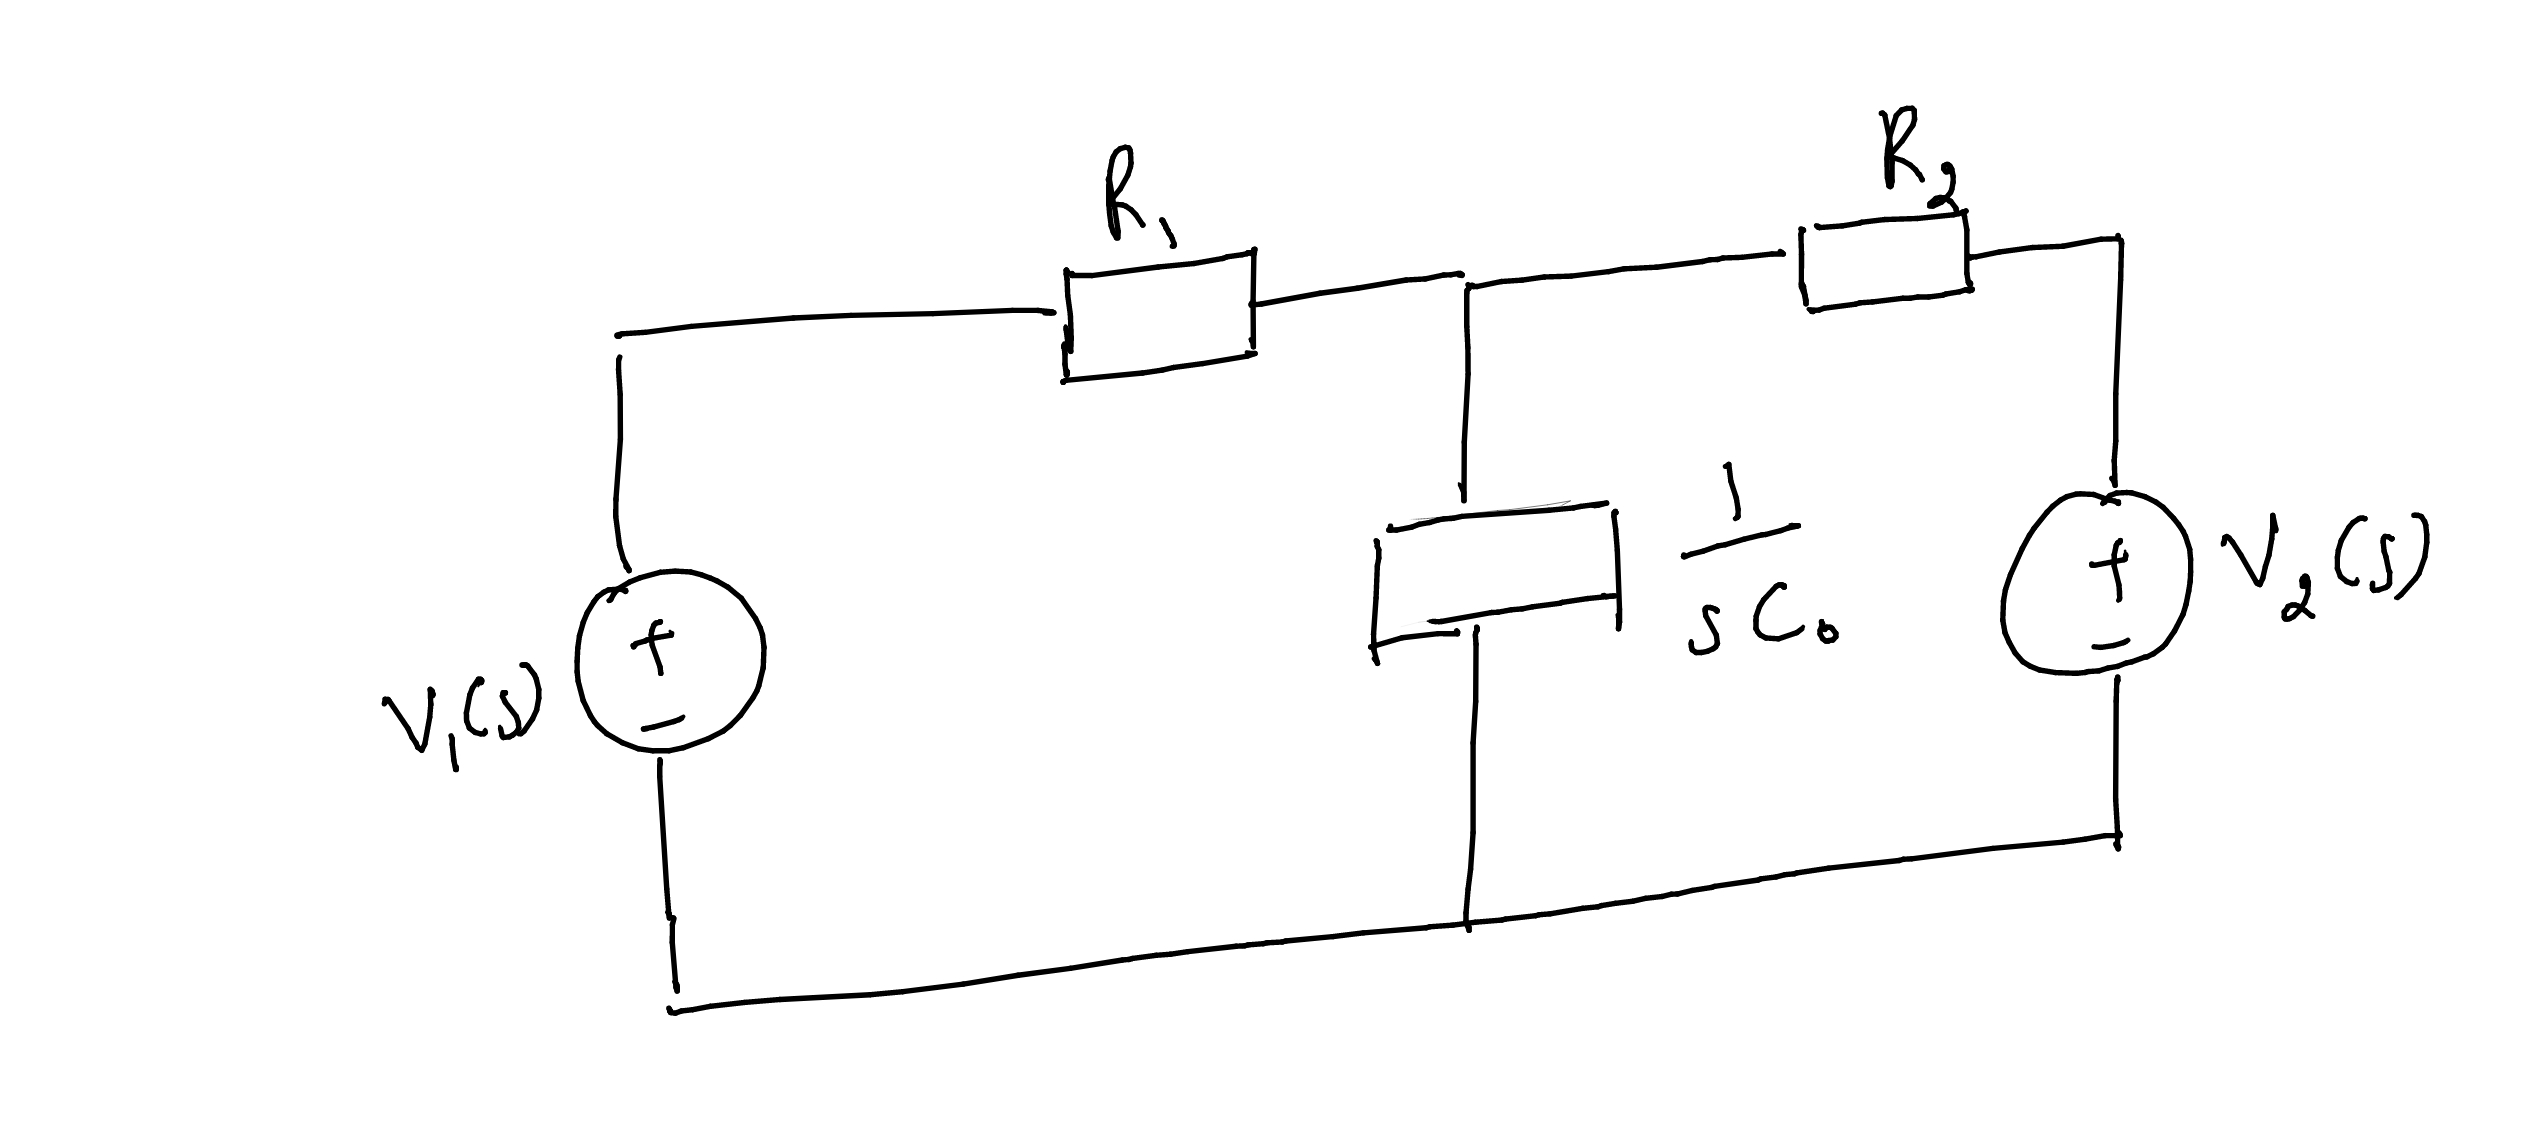
\includegraphics[width=\columnwidth]{Figs/lap-ckt.jpg}
			\caption{}
			\label{fig:lap-ckt}
\end{figure}
		where 
		\begin{align}
			u(t) \system{L} V_1(s)
			\\
			2u(t) \system{L} V_2(s)
		\end{align}
		Find the voltage across the capacitor $V_{C_0}(s)$.\\
	\solution From the earlier proved results,
	  \begin{align}
	    V_1(s) &= \mathcal{L}\brak{u(t)} \\
	           &= \frac{1}{s} \\
	    V_2(s) &= \mathcal{L}\brak{2u(t)} \\
		   &= \frac{2}{s}
	  \end{align}
	   Note that ROC here is $Re\cbrak{s} > 0$. \\
	  And the let the ends of resistive capacitor has voltages of $V_{C_0}$ and $0$. The same can be seen in figure $\ref{Fig-lap-ckt_2}$,
	  \begin{figure}[!ht] 
		\begin{center}
	         \begin{circuitikz}
			\draw (0,0)node[left]{$0$} 
			to [V,l_=$V_1(s)$](0,3)node[left]{$V_{1}$}
			to [generic ,l_ = $1 \Omega$](4,3)
			to [generic,l_ = $2 \Omega$](8,3)
                        ;
			\draw (8,0) node[below]{$0$}
			to [V,l_ = $V_2(s)$](8,3)node[above]{$V_2$}
                        ;
			\draw (4,3) node[above]{$V_{C_0}$}
			to [capacitor,l_ = $\frac{1}{sC_{0}}$](4,0) node[below]{$0$}
			;
			\draw (0,0)
			to [short] (8,0)
			;	
	        \end{circuitikz}
	       \end{center}
	       \caption{}
	       \label{Fig-lap-ckt_2}
          \end{figure} 
        If we apply Kirchoff's Junction law,
	 \begin{align}
		 \frac{V_{C_0} - V_1(s)}{1} + \frac{V_{C_0} - 0}{\frac{1}{sC_0}} \nonumber \\ + \frac{V_{C_0} - V_2(s)}{2}  &= 0 \\
		 V_{C_0}(s)\brak{\frac{3}{2} +sC_0} &= V_1(s) +  \frac{V_2(s)}{2} 
	 \end{align}
 Substituting $V_1(s), V_2(s)$ and $C_0$, you will get
          \begin{align}
		  V_{C_0}(s) &= \frac{4}{s\brak{3 +2x10^{-6}s}}\label{eq:lap-V_c}
	  \end{align}
	\item Find $v_{C_0}(t)$.  Plot using python.\\
	 \solution Now we can find the voltage of capacitor in time domain using inverse laplace transform,
	   \begin{align}
		   v_{C_0}(t) &= \mathcal{L}^{-1}\sbrak{\frac{4}{s\brak{3 +2x10^{-6}s}}} \\
			      &= \mathcal{L}^{-1}\sbrak{\frac{4}{3}\sbrak{\frac{1}{s} - \frac{1}{10^{-6}s + \frac{3}{2}}}} \\
			      &= \frac{4}{3}\mathcal{L}^{-1}\sbrak{\frac{1}{s}} - \frac{4}{3}\mathcal{L}^{-1}\sbrak{\frac{1}{s + \frac{3x10^6}{2}}} \\
			      &= \frac{4}{3}\brak{ u(t) - u(t)e^{-\frac{3x10^6t}{2}}} \\
		   \implies v_{C_0}(t) &= \frac{4}{3}\brak{1 - e^{-\frac{3t}{2}\text{x}10^6}}u(t)
	   \end{align}
	   Note that the ROC here is $Re\cbrak{s} > 0$.\\
	   The plot $\ref{Fig:V_c}$ of the same can be viewed using the python code in the following link,
	 \begin{lstlisting}
wget https://github.com/Charanyash/EE3900-Digital_Signal_Processing/tree/master/Circuits%20and%20Transforms/Codes/2.7.py
         \end{lstlisting}
Then run the following command,
      \begin{lstlisting}
python3 2.7.py
      \end{lstlisting}
      \begin{figure}[ht!]
	       \centering
	       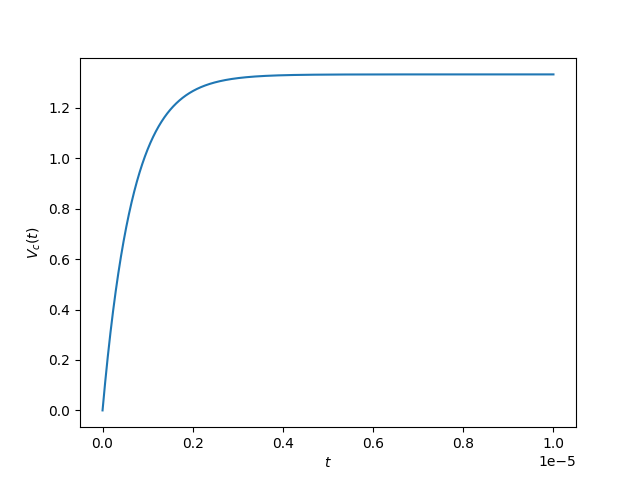
\includegraphics[width = \columnwidth]{Figs/2.7.png}
	       \caption{The plot of $V_c(t)$ vs $t$}
	       \label{Fig:V_c}
     \end{figure}	   
	\item Verify your result using ngspice.\\
	 \solution Download the codes from the below links, 
	   \begin{lstlisting}
wget  https://github.com/Charanyash/EE3900-Digital_Signal_Processing/tree/master/Circuits%20and%20Transforms/Codes/2.8.cir
wget https://github.com/Charanyash/EE3900-Digital_Signal_Processing/tree/master/Circuits%20and%20Transforms/Codes/2.8.py
           \end{lstlisting}
	   Then run the following command,
	\begin{lstlisting}
ngspice 2.8.cir
python3 2.8.py
	\end{lstlisting}
	\begin{figure}
	  \centering
	  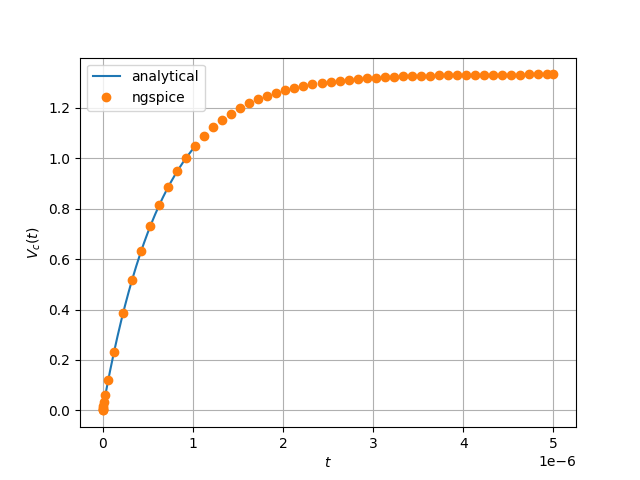
\includegraphics[width = \columnwidth]{Figs/2.8.png}
	  \caption{The plot of $V_c(t)$ vs $t$ using ngspice}
	  \label{Fig:V_c_ngspice}
	\end{figure}
       \item Obtain Fig. 
			$\ref{fig:lap-ckt}$
			using the equivalent differential equation.\\
	\solution Using Kirchoff's Junction Law in $\ref{fig:ckt}$,
	  \begin{align}
		  \frac{v_c(t) - v_1(t)}{1} + \frac{v_c(t) - v_2(t)}{2} + \frac{dq}{dt} &= 0 \label{eq:ckt_jun}
	  \end{align}
	  where $q(t)$ is the charge on capacitor. And can be written as ,
	   \begin{align}
		   q_c(t) &= Cv_c(t)  \label{eq:q_C}
	   \end{align}
	   Now applying laplace transform of $\eqref{eq:ckt_jun}$ using $\eqref{eq:q_C}$,
	   \begin{align}
		   \brak{V_c(s) - V_1(s)} + \frac{1}{2}\brak{V_c(s) - V_2(s)}  \nonumber \\ + C\brak{sV_c(s) - v_c(0^-)} &= 0
	   \end{align}
	   We know,
	    \begin{align}
	        v_c(0^-) = v_c(0) = 0
            \end{align}
            Using that,
	     \begin{align}
		 \frac{V_{C_0} - V_1(s)}{1} + \frac{V_{C_0} - 0}{\frac{1}{sC_0}} + \frac{V_{C_0} - V_2(s)}{2}  &= 0 
	     \end{align}
	     With this equation, we can write the equivalent resistive circuit as shown in Fig $\ref{fig:lap-ckt}$. 
\end{enumerate}
 \section{Initial Conditions}
\begin{enumerate}[label=\arabic*.,ref=\thesection.\theenumi]
\numberwithin{equation}{section}
\item Find $q_2$ in Fig. 
			$\ref{fig:ckt}$. \\
 \solution After closing switch at $Q$ for long time the circuit looks like $\ref{fig:q_2}$,
 
 \begin{figure}[!ht]
	  \begin{center}
	   \begin{circuitikz}
		   \draw (0,0) node[left]{$0$}
	      to [short](0,3)node[above]{$0$}
	      to [R,l_ = $1 \Omega$](4,3)node[above]{$V_c$}
	      to [R,l_ = $ 2 \Omega$](8,3)node[right]{$2$}
	      to [battery1 , l_= $2 V$](8,0) node[right]{$0$}
	      to [short] (0,0)
	      ;
	      \draw(4,3)
	      to [short,*-o](4,1.75) node[right]{$+$} 
	      ;
	      \draw(4,1.25)
	      to [short,*-o](4,0) node[right]{$-$}
	      ;	
            \end{circuitikz}
	   \end{center}
	   \caption{}
	   \label{fig:q_2}
\end{figure}
Now we will use Kirchoff's Junction Law in this circuit,
 \begin{align}
	 \frac{V_c -0}{1} + &\frac{V_c - 2}{2} = 0 \\
	 \implies V_c &= \frac{2}{3}V
 \end{align}
And the charge on the capacitor will be,
   \begin{align}
	 q_2 = \frac{2}{3} \mu C
   \end{align}
\item Draw the equivalent $s$-domain resistive circuit when S is switched to position Q.  Use variables $R_1, R_2, C_0$ for the passive elements.
Use latex-tikz.
		$\label{prob:init}$ \\
		\solution The equivalent $s$-domain resistive circuit looks like $\ref{fig:lap-ckt_q_2}$.
		\begin{figure}[!ht]
		\begin{center}
		\begin{circuitikz}
			\draw (0,0) 
			to [short] (0,3)node[left]{$0$}
			to [generic,l_=$R_1$] (4,3)
			to [generic,l_=$R_2$] (8,3)
			to [V,l_ = $V_2(s)$](8,0)
			;
			\draw (4,3) node[above]{$V_c(s)$}
			to [capacitor,l_ = $\frac{1}{sC_o}$](4,1.75)
			to [V, l_ = $\frac{4}{3s}$](4,0)
			;
			\draw(0,0)
			to [short](8,0)
			;
		\end{circuitikz}
		\end{center}
		\caption{Circuit after closing switch to Q in s-domain}
		\label{fig:lap-ckt_q_2}
		\end{figure}
		The battery $\frac{4}{3s}$ is added series to $C_0$ in s- domain by taking consideration of initial charge on capacitor $q_1 = \frac{4}{3} \mu C$ before closing switch to Q. 
	\item $V_{C_0}(s)$ = ?\\
		\solution Apply kirchoff's junction law in the s-domain circuit $\ref{fig:lap-ckt_q_2}$,taking $R_1 = 1 \Omega$ and $R_2 = 2 \Omega$
		    \begin{align}
			    \frac{V_{C_0}(s) - 0}{1} + \frac{V_{C_0}(s) - \frac{4}{3s}}{\frac{1}{sC_0}} &+ \frac{V_{C_0}(s) - V_2(s)}{2} = 0 \\
			    \implies V_{C_0}(s)\brak{\frac{3}{2} + sC_0} &= \frac{V_2(s)}{2} + \frac{4C_0}{3} \\
			    \implies V_{C_0}(s) &= \frac{\frac{1}{s} + \frac{4C_0}{3}}{\frac{3}{2} + sC_0} \\ 
		    \therefore V_{C_0}(s) = \frac{2\brak{3 + 4sC_0}}{3s\brak{3 + 2sC_0}}
		     \end{align}
	\item $v_{C_0}(t)$ = ? Plot using python.\\
	 \solution We can obtain the potential difference across the capacitor in time domain by applying inverse laplace transform under right ROC conditions,
	   \begin{align}
		   v_{C_0}(t) &= \mathcal{L}^{-1}\sbrak{\frac{2\brak{3 + 4sC_0}}{3s\brak{3 + 2sC_0}}} \\
			      &= \mathcal{L}^{-1}\sbrak{\frac{2}{3s} + \frac{4C_0}{3\brak{3 + 2sC_0}}} \\
			      &= \mathcal{L}^{-1}\sbrak{\frac{2}{3s}} + \mathcal{L}^{-1}\sbrak{\frac{4C_0}{3\brak{3 + 2sC_0}}}
           \end{align}
              With ROC condition $Re\cbrak{s} > 0$,
	       \begin{align}
		       v_{C_0}(t) &= \frac{2u(t)}{3} + \frac{2u(t)}{3}e^{-\frac{3}{2C_0}}
	       \end{align}
            Substituting $C_0 = 1 \mu F$,
	       \begin{align}
		       v_{C_0}(t) &= \frac{2}{3}\brak{1 + e^{-\frac{3x 10^6}{2}}}u(t)\label{eq:V_C_2}
	       \end{align}
             We can verify the same using the python code from the below link,
	      \begin{lstlisting} 
wget  https://github.com/Charanyash/EE3900-Digital_Signal_Processing/tree/master/Circuits%20and%20Transforms/Codes/3.4.py
	      \end{lstlisting}
	      Then run the following command,
	       \begin{lstlisting}
wget  python3 3.4.py
	       \end{lstlisting}
	       
		\begin{figure}[!ht]
			\centering
			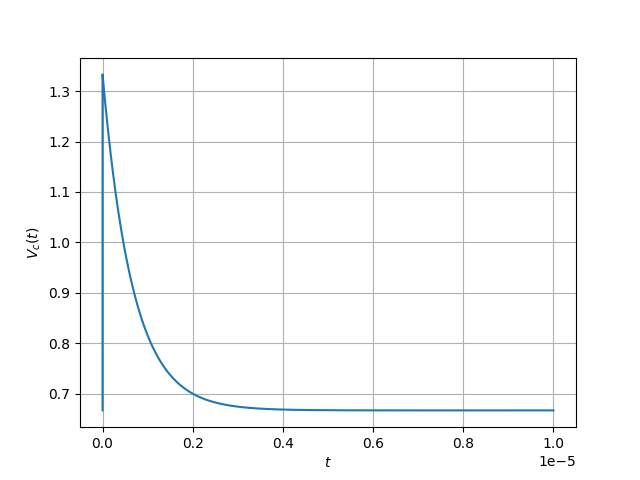
\includegraphics[width=\columnwidth]{Figs/3.4.png}
			\caption{The plot of $V_c(t)$ vs $t$}
			\label{fig:V_c_t_2}
\end{figure}
	\item Verify your result using ngspice. \\
	  \solution 
	     Download the codes from the below links
	      \begin{lstlisting}
wget  https://github.com/Charanyash/EE3900-Digital_Signal_Processing/tree/master/Circuits%20and%20Transforms/Codes/3.5.py	      
wget  https://github.com/Charanyash/EE3900-Digital_Signal_Processing/tree/master/Circuits%20and%20Transforms/Codes/3.5.cir
              \end{lstlisting}
    Then run the following commands,
     \begin{lstlisting}
ngspice 3.5.cir
python3 3.5.py
    \end{lstlisting}
		\begin{figure}[!ht]
			\centering
			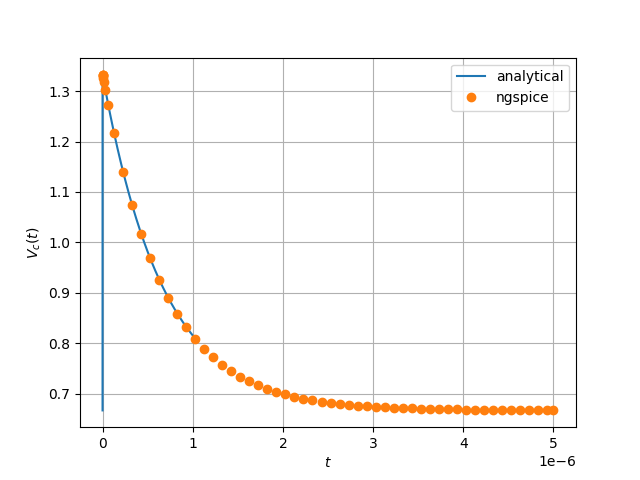
\includegraphics[width=\columnwidth]{Figs/3.5.png}
			\caption{The plot of $V_c(t)$ vs $t$ using ngspice}
			\label{fig:ngspice_2}
\end{figure}
\item Find $v_{C_0}(0-), v_{C_0}(0+)$ and  $v_{C_0}(\infty) $.\\
	\solution In that case when $t < 0$ switch is not closed to Q so the circuit will be in steady state $(\text{switch at P})$,
	  \begin{align}
		  v_{C_0}(0-) &= \sbrak{\frac{4}{3}\brak{1 - e^{-\frac{3x 10^6}{2}}}u(t)}_{t = \infty} \\
			      &= \frac{4}{3}V
	   \end{align}
	   And for $t = 0+$ and $t = \infty$, we can use $\eqref{eq:V_C_2}$,
	    \begin{align}
		    v_{C_0}(0+) &= \frac{4}{3}V \\
		    v_{C_0}(\infty) &= \frac{2}{3}V
	    \end{align}
\item Obtain the Fig.  in problem 
		$\ref{prob:init}$
			using the equivalent differential equation.\\
	\solution Using Kirchoff's Junction Law ,
	  \begin{align}
		  \frac{v_c(t) - v_1(t)}{1} + \frac{v_c(t) - v_2(t)}{2} + \frac{dq}{dt} &= 0
	  \end{align}
	  where $q(t)$ is the charge on capacitor. And can be written as ,
	   \begin{align}
		   q_c(t) &= Cv_c(t)  
	   \end{align}
	   Now applying laplace transform ,
	   \begin{align}
		   \brak{V_c(s) - V_1(s)} + \frac{1}{2}\brak{V_c(s) - V_2(s)}  \nonumber \\ + C\brak{sV_c(s) - v_c(0^-)} &= 0
	   \end{align}
	   We know,
	    \begin{align}
		    v_c(0^-) = \frac{4}{3}V
            \end{align}
            Using that,
	     \begin{align}
		     \frac{V_{C_0} - V_1(s)}{R_1} + \frac{V_{C_0} - \frac{4}{3s}}{\frac{1}{sC_0}} + \frac{V_{C_0} - V_2(s)}{R_2}  &= 0 
	     \end{align}
	     With this equation, we can write the equivalent resistive circuit as shown in Fig $\ref{fig:lap-ckt_q_2}$. 
 \end{enumerate}
\section{Bilinear Transform}
\begin{enumerate}[label=\arabic*.,ref=\thesection.\theenumi]
\numberwithin{equation}{section}
\item In Fig. 
			\ref{fig:ckt},
			consider the case when $S$ is switched to $Q$ right in the beginning. Formulate the differential equation.
		\item Find $H(s)$ considering the ouput voltage at the capacitor.
		\item Plot $H(s)$.  What kind of filter is it?
		\item Using trapezoidal rule for integration, formulate the difference equation
			by considering 
		\begin{align}
			y(n) = y(t)\vert_{t=n}
		\end{align}
	\item Find $H(z)$.
	\item How can you obtain $H(z)$ from $H(s)$?
	\end{enumerate}

\end{document}
